\documentclass[11pt]{article}
\usepackage[top=1in, bottom=0.5in, left=1in, right=1in]{geometry}
\usepackage[T1]{fontenc}
\usepackage[polish]{babel}
\usepackage[utf8]{inputenc}
\usepackage{lmodern}
\selectlanguage{polish}
\usepackage{graphicx}
\begin{document}
\title{Laboratorium 4}
\author{Jan Seredyński}
\date{\today}
\maketitle

\section{Wstęp}
Zadaniem laboratorium jest pomiar czasu wykonania operacji wypelnienia tablicy asocjacyjnej (słownika). Do wykonania analizy zstosowałem wcześniej przygotowaną listę dwukierunkową(nie opartą na tablicy).


\section{Schematy odpowiednich struktur}

Lista dwukierunkowa
\includegraphics[width=5in]{lista2_1.png} 
\par\vspace{\baselineskip}
\hrule
\par\vspace{\baselineskip}


\section{Wydajność listy}
Podczas poprzednich laboratoriow przygotowałem implementacje listy dwukierunkowej(kolor fioletowy na wykresie, której zlożoność obliczeniowa wynosi O(n) przy wypelnianiu jej o jeden element(przykład stosu)
\par\vspace{\baselineskip}

\includegraphics[width=4.5in]{3stos_dyn_o_200ilista.png}

\section{Wydajność słownika}
Wykorzystałem metode łańcuchową transformacji kluczowej, której idee pokazuje obraz poniżej.
\par\vspace{\baselineskip}
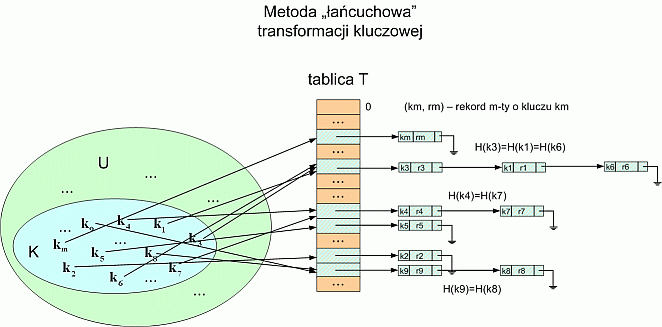
\includegraphics[width=5in]{lancuchowa.png}\\\
W mojej implementacji złożoność obliczeniowa słownika wynosi $O(n^2)$), ponieważ algorytm żeby dostać się do odpowiedniego elementu kX na liscie potrzebuje najpierw wypopowac elementy na tymczasową liste, a gdy go znajdzie(i doda/odczyta) to następnie musi zpushować je spowrotem z tymczasowej listy na oryginalną.\\\
To doprowadza do momentu, w którym otrzymujemy liniowy wykres dla popowania i pushowania, więc ich iloczyn daje nam funkcję kwadratową.\\\
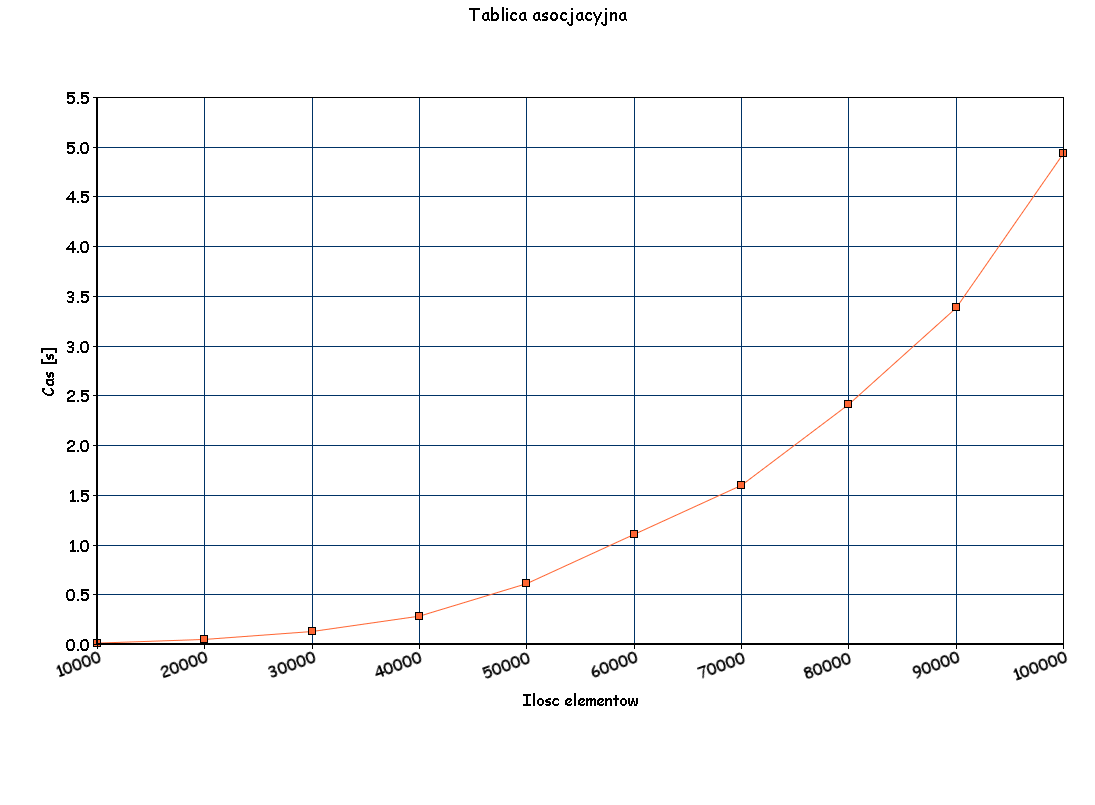
\includegraphics[width=6in]{slownik.png}


\section{Podsumowanie}
Mógłbym ulepszyć moją tablice asocjacyjną poprzez zrobienie jej na liscie opartej na tablicy i zastosowainu sortowania binarnego.
Kolejnym ulepszeniem byłoby ulepszenie mojej implementacji listy, tak aby mogła wyszukiwać elementy w liscie bez potrzeby popowania wczesniejszych elementów.
\end{document}